%%%%%%%%%%%%%%%%%%%%%%% file template.tex %%%%%%%%%%%%%%%%%%%%%%%%%
%
% This is a general template file for the LaTeX package SVJour3
% for Springer journals.          Springer Heidelberg 2010/09/16
%
% Copy it to a new file with a new name and use it as the basis
% for your article. Delete % signs as needed.
%
% This template includes a few options for different layouts and
% content for various journals. Please consult a previous issue of
% your journal as needed.
%
%%%%%%%%%%%%%%%%%%%%%%%%%%%%%%%%%%%%%%%%%%%%%%%%%%%%%%%%%%%%%%%%%%%
%
% First comes an example EPS file -- just ignore it and
% proceed on the \documentclass line
% your LaTeX will extract the file if required
\begin{filecontents*}{example.eps}
%!PS-Adobe-3.0 EPSF-3.0
%%BoundingBox: 19 19 221 221
%%CreationDate: Mon Sep 29 1997
%%Creator: programmed by hand (JK)
%%EndComments
gsave
newpath
  20 20 moveto
  20 220 lineto
  220 220 lineto
  220 20 lineto
closepath
2 setlinewidth
gsave
  .4 setgray fill
grestore
stroke
grestore
\end{filecontents*}
%
\RequirePackage{fix-cm}
%
%\documentclass{svjour3}                     % onecolumn (standard format)
%\documentclass[smallcondensed]{svjour3}     % onecolumn (ditto)
\documentclass[smallextended]{svjour3}       % onecolumn (second format)
%\documentclass[twocolumn]{svjour3}          % twocolumn
%
\smartqed  % flush right qed marks, e.g. at end of proof
%
%\usepackage{units}
%\usepackage{multirow}
%\usepackage{amstext}
%\usepackage{amsmath}
%\usepackage{amssymb}
%\usepackage{amsfonts}
\usepackage{enumerate}
\usepackage{cite}
%\usepackage{natbib}
%\usepackage{amsthm}
\usepackage{array,arydshln}
\usepackage[pdftex]{graphicx}
\usepackage{rotating}
\usepackage{ifpdf}
%\usepackage{epsfig}
\usepackage[all]{xy}
\usepackage{latexsym}
\usepackage[hidelinks]{hyperref}
\usepackage{color}
%
\usepackage{mathptmx}      % use Times fonts if available on your TeX system
%
% insert here the call for the packages your document requires
%\usepackage{latexsym}
% etc.
%
% please place your own definitions here and don't use \def but
% \newcommand{}{}
%
% Insert the name of "your journal" with
% \journalname{myjournal}
%
\begin{document}

\title{Development of an Algorithm Improving Label Arrangements in Offset Printing}
\subtitle{Do you have a subtitle?\\ If so, write it here}

%\titlerunning{Short form of title}        % if too long for running head

\author{First Author         \and
        Second Author %etc.
}

%\authorrunning{Short form of author list} % if too long for running head

\institute{F. Author \at
              first address \\
              Tel.: +123-45-678910\\
              Fax: +123-45-678910\\
              \email{fauthor@example.com}           %  \\
%             \emph{Present address:} of F. Author  %  if needed
           \and
           S. Author \at
              second address
}

\date{Received: date / Accepted: date}
% The correct dates will be entered by the editor


\maketitle

\thanks{}

\begin{abstract}
One of the most classic problems in the manufacturing industry is inventory processing. 
The best method to solve the problem is not to make any inventory. 
There is a way to effectively reduce inventory by merely changing the array of the pieces on the printing plates in the offset printing. 
It is setting an upper limit of acceptable for each plate and carrying out complete enumeration. 
These method reduce the accuracy, but dramatically reduces the operating time of the algorithm. 
The strength of this method lies in the fact that there is only change the arrangement of the pieces inside the plates.
%subject classification numbers as needed.
\keywords{First keyword \and Second keyword \and More}
% \PACS{PACS code1 \and PACS code2 \and more}
% \subclass{MSC code1 \and MSC code2 \and more}
\end{abstract}

\section{Introduction}\label{sec:intro}
A combinations with repetition is the number of cases, where $k$ elements are selected from among different $n$ elements allowing repetition [1]. 
It is indicated with the symbol $_{n}H_{k}$ and the following is established.
\begin{equation}
	_{n}H_{k} = _{n+k-1}C_{k} = \frac{(n+k-1)!}{(n-1)!k!}
\end{equation}
For instance, the combinations with repetition $_{2}H_{4}$ to select four elements from among two elements A and B comprises the following five cases.
\begin{enumerate}[(1)]
	\item $\textrm{[A, A, A, A]}$ : a list consisting of four A's
	\item $\textrm{[A, A, A, B]}$ : a list consisting of three A's and one B
	\item $\textrm{[A, A, B, B]}$ : a list consisting of two each of A's and B's
	\item $\textrm{[A, B, B, B]}$ : a list consisting of one A and three B's
	\item $\textrm{[B, B, B, B]}$ : a list consisting of four B's
\end{enumerate}
Among the above cases, if we want to obtain three A's and nine B's, then we can choose $[\textrm{A, B, B, B}] \times 3$. 
Let us consider the following.
\begin{equation}
	\textrm{[A, A, B, B]} \times 1 + \textrm{[A, B, B, B]} \times 1 + \textrm{[B, B, B, B]} \times 1
\end{equation}
In this case, we can get the three A's and nine B's. 
However, the former case seems to be a ‘Better’ because making three different lists is inefficient. 
Let us examine another case.
\begin{equation}
\textrm{[A, A, A, A]} \times 1 + \textrm{[B, B, B, B]} \times 3 - \textrm{[A]} \times 1 - \textrm{[B]} \times 3
\end{equation}
$\textrm{[A, B, B, B]} \times 3$ also seems to be 'Better' because there is no loss. Under the following conditions, $\textrm{[A, B, B, B]} \times 3$ is the ‘Best’ method.
\begin{enumerate}[(1)]
	\item Minimize the number of list.
	\item Minimize the loss of lists.
\end{enumerate}
Offset printing, also called offset lithography, or litho-offset, in commercial printing, 
widely used printing technique in which the inked image on a printing plate is printed on a rubber cylinder and then transferred (i.e., offset) to paper or other material. 
The rubber cylinder gives great flexibility, permitting printing on wood, cloth, metal, leather, and rough paper (see Fig.1) [2].

Offset lithography is one of the most common ways of creating printed materials. A few of its common applications include: newspapers, magazines, brochures, stationery, and books. Compared to other printing methods, offset printing is best suited for economically producing large volumes of high quality prints in a manner that requires little maintenance [3]. Therefore, how to make the initial plates is an important issue. Above example means that what is the best arrangement in such print method.

In the past, production was based on ordering of products from companies. For instance, apparel companies stocked popular products in warehouses. If the companies didn't have inventory, then consumers could not obtain rare sized or unpopular products. However, as the Internet market has became popular, the production systems have been changed into systems. Factories do not produce products based on their prediction of consumption but do produce only ordered products.

World Komax is a company that produces labels using the offset printing. The labels refer to stickers containing bar-codes attached to garments or shoes as follows (see Fig.2). Each bar-code in the label contains fixed information such as product names and colors, and variable information such as the date of manufacture.

Since the program of World Komax is not suitable for small quantity batch productions, the number of labels loss increased compared to the past.

Section 2 of this paper will describe the process of label printing using offsets. The modeling of the problem will be carried out in Section 3, and examples to help the understanding of the problem will be prepared in Section 4. The final results of the algorithm will be described in Section 5. 


\section{Offset label printing process}\label{sec:Offset}

\subsection{Label printing process}\label{subsec:LabelPrinting}
Prior to describing the label printing process, we define the following terms first.
\begin{enumerate}[*]
	\item {\bf Plate} : A printing plate for the offset printing (see Fig.3)
	\item {\bf Loss} : The number of labels printed in excess of the order-quantity
\end{enumerate}

The offset label printing process is as follows. At first, we receive orders from customers. The order includes many types of labels to be printed and order-quantities by type (see Fig. 4). Thereafter, offset printing plates are made. Many types of labels are placed on each plate so that many labels are printed at one printing. When the plates have been made, the printing operation is carried out so that individual labels are produced in quantities not smaller than the order-quantities using individual plates. As the final process, the sheets are cut to the sizes of labels and labels are collected by type.

\subsection{Major points for cost saving}\label{subsec:CostSave}
The constraint conditions and major points that will be considered in this paper for cost saving are as follows. First, one type of label should be placed on one plate only. This is to prevent different types of labels from being mixed when collected by type after the printed sheets are cut. Meanwhile, the total number of labels placed on each plate is also constant because the sizes of individual plates are constant and the sizes of labels in one order are also constant. In addition, the number of plates should be minimized as little as possible because plates are made using molds and the costs are high. Finally, the losses of labels printed should be minimized because bar-codes which are used only one time are printed in the labels and if the inventory remains, they cannot be used and should be entirely discarded.

\subsection{Sorting report output program}\label{subsec:SortProgram}
Plate fabrication and the use of printing paper incur costs. In order to reduce the costs, order details are inputted to output appropriate methods to place labels on the plate as sorting reports. The plate makers produce plates according to the instructions in the sorting reports (see Fig. 4).

Since the existing sorting report output method was not suitable for small quantity batch production systems, the algorithm should be improved. Therefore, this study was conducted to develop new algorithms suitable for small quantity batch production systems too.







\paragraph{Paragraph headings} Use paragraph headings as needed.
\begin{equation}
a^2+b^2=c^2
\end{equation}

% For one-column wide figures use
\begin{figure}
% Use the relevant command to insert your figure file.
% For example, with the graphicx package use
  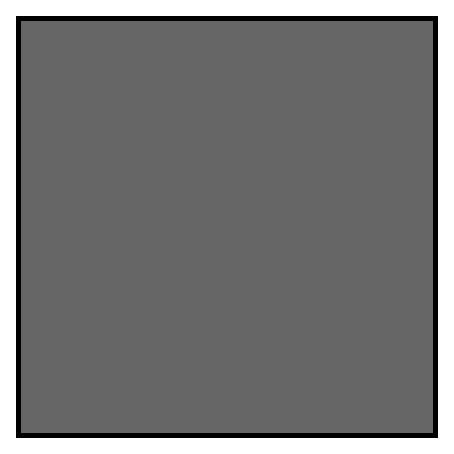
\includegraphics{example.eps}
% figure caption is below the figure
\caption{Please write your figure caption here}
\label{fig:1}       % Give a unique label
\end{figure}
%
% For two-column wide figures use
\begin{figure*}
% Use the relevant command to insert your figure file.
% For example, with the graphicx package use
  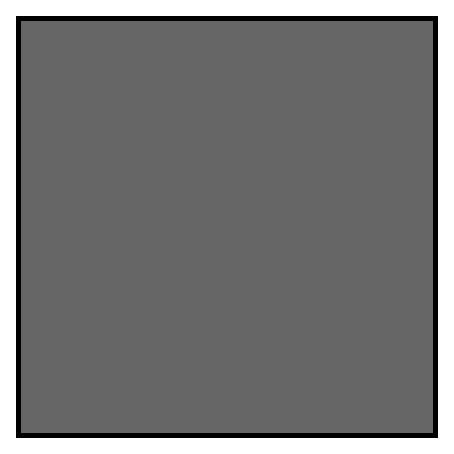
\includegraphics[width=0.75\textwidth]{example.eps}
% figure caption is below the figure
\caption{Please write your figure caption here}
\label{fig:2}       % Give a unique label
\end{figure*}
%
% For tables use
\begin{table}
% table caption is above the table
\caption{Please write your table caption here}
\label{tab:1}       % Give a unique label
% For LaTeX tables use
\begin{tabular}{lll}
\hline\noalign{\smallskip}
first & second & third  \\
\noalign{\smallskip}\hline\noalign{\smallskip}
number & number & number \\
number & number & number \\
\noalign{\smallskip}\hline
\end{tabular}
\end{table}


%\begin{acknowledgements}
%If you'd like to thank anyone, place your comments here
%and remove the percent signs.
%\end{acknowledgements}

% BibTeX users please use one of
%\bibliographystyle{spbasic}      % basic style, author-year citations
%\bibliographystyle{spmpsci}      % mathematics and physical sciences
%\bibliographystyle{spphys}       % APS-like style for physics
%\bibliography{}   % name your BibTeX data base

% Non-BibTeX users please use
\begin{thebibliography}{}
%
% and use \bibitem to create references. Consult the Instructions
% for authors for reference list style.
%
\bibitem{RefJ}
% Format for Journal Reference
Author, Article title, Journal, Volume, page numbers (year)
% Format for books
\bibitem{RefB}
Author, Book title, page numbers. Publisher, place (year)
% etc
\end{thebibliography}

\end{document}
% end of file template.tex

